% ============================================================================ EVALUATE
\section{Evaluating a Design}\label{sec:evaluate}

The evaluated design is the embedded regulator (Z1), the integration of the reference
framework~\cite{Krishnakumar2026DVPD}, at the design point of Table~\ref{tab:spec}. It runs in the
production state, with the implemented input decoupling, under cooling~A.
Fig.~\ref{fig:fields}(a), (d) and~(g) show its fields, and the first column of
Table~\ref{tab:compare} gives its numbers.

\subsection{Electrothermal State}\label{sec:evaluate-et}
The fixed point converges in \WrEtItersAZoneWord{} iterations to \PlossAZone~W inside the package, a
package-internal efficiency of \WrEffAZone\,\%. Conversion accounts for \PconvAZone~W, and the
low-side devices alone dissipate \WrPconvLsAZone~W of it (\WrLsShareAZone\,\%). Routing accounts for
\ProuteAZone~W: \WrPintraAZone~W in the cells' own conductors, \WrPhvAZone~W in the package 48-V
network and \WrPringAZone~W in the input capacitors.

The peak, \TmaxAZone\,$^\circ$C, lies in the input-end tier, which holds two high-side devices and
the two flying capacitors. That tier sits farthest from the cold plate: its heat crosses the other
three tiers and the die. The other three tiers peak at \WrTtierTwoAZone, \WrTtierThreeAZone{} and
\WrTtierFourAZone\,$^\circ$C, falling toward the die. The die averages \WrTdieMeanAZone\,$^\circ$C and
peaks at \TdiemaxAZone\,$^\circ$C under its uniform load.

Evaluated with every region at 25\,$^\circ$C, the same ledger returns \WrIsoLoZone~W. An electrical
analysis decoupled from the thermal solution would therefore understate the package loss by
\WrUnderAZone\,\% (\WrRiseAZone~W). The difference is the on-resistance and copper resistivity of
parts that run \WrTlsRiseAZone{} to \WrThsRiseAZone~K above room temperature.

\subsection{Input Decoupling}\label{sec:evaluate-decap}
Capacitance inside the stack does not lower the RMS factor $k_{\mathrm{rms}}$ enough, and neither
does interleaving or a ring alone, so the implemented decoupling (Section~\ref{sec:scenarios})
combines the last two. With the cells in phase and no input capacitance, a port model of the package network
gives $k_{\mathrm{rms}} = \WrKsync$.

Charge balance asks for only \WrCchargeOneV~\textmu F per cell for 1~V of input ripple. A circuit
model of the package loop says otherwise. It includes the loop's inductance, \WrLloop~pH nominal
within \WrLloopLo--\WrLloopHi~pH, and the capacitors' series resistance, series inductance and bias
derating. In that model $k_{\mathrm{rms}}$ falls slowly with capacitance: $k_{\mathrm{rms}} \le 1.2$
needs about \WrCkTwelve~\textmu F per cell at 100~pH.

The embedded stack has no room for that. The gaps between cells hold \WrGapCapsPerCell{} capacitors
per cell, 0402 100-V X7R parts, the largest such part rated to 125\,$^\circ$C. Their few nanofarads
resonate with the package inductance and raise $k_{\mathrm{rms}}$ to \WrKgap{}, and to \WrKgapHi{} at
the worst inductance of the band. A ring of \FrDecapN{} capacitors outside the cell grid, 1206 100-V
X7S parts, holds \FrDecapCtot~\textmu F at 48~V and 105\,$^\circ$C. On its own it gives
$k_{\mathrm{rms}} = \WrKring$, because the package inductance separates it from the cells.
Interleaving the cells' clocks on its own gives \WrKinter.

In the implemented decoupling, \FrDecapPhases{} clock phases form two interleaved
\FrDecapGroupWord-phase groups on a checkerboard, the second offset by half a phase step. With the ring
they reach $k_{\mathrm{rms}} = \WrKrms$, and \WrKrmsLo--\WrKrmsHi{} over the inductance band. An ideal
\FrDseOptM-phase spread with the ring would reach only \WrKspread: the sheet next to each cell still
carries that cell's own pulse.

The implemented decoupling costs \WrDecapCoupledA~W against ideal decoupling in the coupled case.
Of this, \WrHotLoop~W is dissipated in the cells' own input loops, which carry the bare pulse
whatever sits outside the cell. Bare decoupling would cost \RiseSoneZone~W more than ideal
decoupling. It would also put \WrBgaBareAtNmaxZone~A on each 48-V ball even at the legal maximum of
\WrBgaNmax{} balls per rail, beyond the per-ball target. The interleaving is therefore a requirement
on the converter's control, not an option.

\subsection{Package Interface}\label{sec:evaluate-bga}
At the implemented waveform the ball rule of Section~\ref{sec:ledger} gives the 48-V field of Z1
\WrBgaNZone{} balls per rail, the smallest legal count, each carrying \WrBgaIZone~A, on \WrBgaFracZone\,\% of the
\MthSitesFull{} sites. The static 1-V drop from the converter output to the die is
\VdropAZone~mV per rail, within the \MthLimDrop-mV limit.

\subsection{Mechanical State}\label{sec:evaluate-mech}
The die warps by \WarpAZone~\textmu m peak to valley. The largest relative displacement across the
ball layer lies at a corner of the array, $\du = \DuAZone$~\textmu m. The critical joint is that
corner or its mirror image, at $T_{\mathrm{sj}} = \MvTsjAZone\,^\circ$C. It accumulates
$\deps = \MvEpsAZone\times10^{-3}$ per cycle under the production law, with a numerical uncertainty
of \MvEpsUrelAZone\,\%, and \MvEpsLoAZone$\times10^{-3}$ under the lowest law of the band.

Of the other interconnect layers, the \WrHIfUm-\textmu m die-to-converter microbumps carry the
largest driver: $\gamma = \WrGamIfAZone\times10^{-3}$ at \WrTIfAZone\,$^\circ$C, about
\WrGamRatioAZoneWord{} times that of the ball of largest $\Delta u$ ($\WrGamBgaAZone\times10^{-3}$).
Section~\ref{sec:compare-joints} explains why these layers are screened rather than ranked.

\subsection{Feasibility}\label{sec:evaluate-feas}
The evaluated design passes every check of the feasibility stage (Table~S19). The GaN junctions
reach $T_{\mathrm{jn}} = \TjAZone\,^\circ$C, \WrGanMarginAZone~K below their \MthLimGan-$^\circ$C
rating. Three limits bind more tightly than that rating. The hotter junction lies
\WrRonMarginAZone~K below \MthLimRonFit\,$^\circ$C, the upper end of the on-resistance fit, beyond
which the loss model would extrapolate. The flying-capacitor tier peaks \WrMlccMarginAZone~K below
its \MthLimMlcc-$^\circ$C class. The hottest joint lies \WrSolderMarginAZone~K inside the range of the
solder laws. Under its uniform load the die peaks \WrDieMarginAZone~K below its
\MthLimDie-$^\circ$C limit. Section~\ref{sec:explore} shows which explored decisions consume these
margins.

\begin{figure*}[!t]
\centering
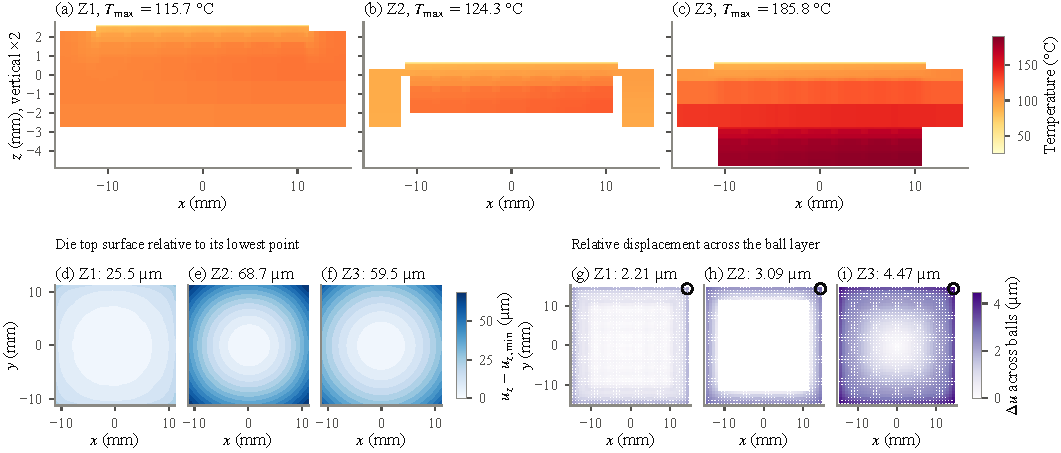
\includegraphics[width=\textwidth]{fig7_fields.pdf}
\caption{Converged fields of the three integrations in the production state (implemented input
decoupling) under cooling~A (one top cold plate). (a)--(c) Temperature on the vertical section
through the middle row of cells (vertical scale doubled; voids left empty; dashed: the
\MthLimGan-$^\circ$C GaN-rating isotherm). (d)--(f) Out-of-plane displacement of the die top surface
relative to its lowest point; its peak-to-valley value is the die warpage. (g)--(i) Relative
in-plane displacement across the ball layer at every legal site. Ring: the joint of largest
$\Delta u$, whose value heads the panel; cross: the critical joint where it is neither that joint
nor its mirror image. Z3 includes its coupled land-side and board-plane redistribution.}
\label{fig:fields}
\end{figure*}
